% Options for packages loaded elsewhere
% Options for packages loaded elsewhere
\PassOptionsToPackage{unicode}{hyperref}
\PassOptionsToPackage{hyphens}{url}
\PassOptionsToPackage{dvipsnames,svgnames,x11names}{xcolor}
%
\documentclass[
  11pt,
  letterpaper,
  DIV=11,
  numbers=noendperiod]{scrartcl}
\usepackage{xcolor}
\usepackage{amsmath,amssymb}
\setcounter{secnumdepth}{-\maxdimen} % remove section numbering
\usepackage{iftex}
\ifPDFTeX
  \usepackage[T1]{fontenc}
  \usepackage[utf8]{inputenc}
  \usepackage{textcomp} % provide euro and other symbols
\else % if luatex or xetex
  \usepackage{unicode-math} % this also loads fontspec
  \defaultfontfeatures{Scale=MatchLowercase}
  \defaultfontfeatures[\rmfamily]{Ligatures=TeX,Scale=1}
\fi
\usepackage{lmodern}
\ifPDFTeX\else
  % xetex/luatex font selection
\fi
% Use upquote if available, for straight quotes in verbatim environments
\IfFileExists{upquote.sty}{\usepackage{upquote}}{}
\IfFileExists{microtype.sty}{% use microtype if available
  \usepackage[]{microtype}
  \UseMicrotypeSet[protrusion]{basicmath} % disable protrusion for tt fonts
}{}
\makeatletter
\@ifundefined{KOMAClassName}{% if non-KOMA class
  \IfFileExists{parskip.sty}{%
    \usepackage{parskip}
  }{% else
    \setlength{\parindent}{0pt}
    \setlength{\parskip}{6pt plus 2pt minus 1pt}}
}{% if KOMA class
  \KOMAoptions{parskip=half}}
\makeatother
% Make \paragraph and \subparagraph free-standing
\makeatletter
\ifx\paragraph\undefined\else
  \let\oldparagraph\paragraph
  \renewcommand{\paragraph}{
    \@ifstar
      \xxxParagraphStar
      \xxxParagraphNoStar
  }
  \newcommand{\xxxParagraphStar}[1]{\oldparagraph*{#1}\mbox{}}
  \newcommand{\xxxParagraphNoStar}[1]{\oldparagraph{#1}\mbox{}}
\fi
\ifx\subparagraph\undefined\else
  \let\oldsubparagraph\subparagraph
  \renewcommand{\subparagraph}{
    \@ifstar
      \xxxSubParagraphStar
      \xxxSubParagraphNoStar
  }
  \newcommand{\xxxSubParagraphStar}[1]{\oldsubparagraph*{#1}\mbox{}}
  \newcommand{\xxxSubParagraphNoStar}[1]{\oldsubparagraph{#1}\mbox{}}
\fi
\makeatother


\usepackage{longtable,booktabs,array}
\usepackage{calc} % for calculating minipage widths
% Correct order of tables after \paragraph or \subparagraph
\usepackage{etoolbox}
\makeatletter
\patchcmd\longtable{\par}{\if@noskipsec\mbox{}\fi\par}{}{}
\makeatother
% Allow footnotes in longtable head/foot
\IfFileExists{footnotehyper.sty}{\usepackage{footnotehyper}}{\usepackage{footnote}}
\makesavenoteenv{longtable}
\usepackage{graphicx}
\makeatletter
\newsavebox\pandoc@box
\newcommand*\pandocbounded[1]{% scales image to fit in text height/width
  \sbox\pandoc@box{#1}%
  \Gscale@div\@tempa{\textheight}{\dimexpr\ht\pandoc@box+\dp\pandoc@box\relax}%
  \Gscale@div\@tempb{\linewidth}{\wd\pandoc@box}%
  \ifdim\@tempb\p@<\@tempa\p@\let\@tempa\@tempb\fi% select the smaller of both
  \ifdim\@tempa\p@<\p@\scalebox{\@tempa}{\usebox\pandoc@box}%
  \else\usebox{\pandoc@box}%
  \fi%
}
% Set default figure placement to htbp
\def\fps@figure{htbp}
\makeatother


% definitions for citeproc citations
\NewDocumentCommand\citeproctext{}{}
\NewDocumentCommand\citeproc{mm}{%
  \begingroup\def\citeproctext{#2}\cite{#1}\endgroup}
\makeatletter
 % allow citations to break across lines
 \let\@cite@ofmt\@firstofone
 % avoid brackets around text for \cite:
 \def\@biblabel#1{}
 \def\@cite#1#2{{#1\if@tempswa , #2\fi}}
\makeatother
\newlength{\cslhangindent}
\setlength{\cslhangindent}{1.5em}
\newlength{\csllabelwidth}
\setlength{\csllabelwidth}{3em}
\newenvironment{CSLReferences}[2] % #1 hanging-indent, #2 entry-spacing
 {\begin{list}{}{%
  \setlength{\itemindent}{0pt}
  \setlength{\leftmargin}{0pt}
  \setlength{\parsep}{0pt}
  % turn on hanging indent if param 1 is 1
  \ifodd #1
   \setlength{\leftmargin}{\cslhangindent}
   \setlength{\itemindent}{-1\cslhangindent}
  \fi
  % set entry spacing
  \setlength{\itemsep}{#2\baselineskip}}}
 {\end{list}}
\usepackage{calc}
\newcommand{\CSLBlock}[1]{\hfill\break\parbox[t]{\linewidth}{\strut\ignorespaces#1\strut}}
\newcommand{\CSLLeftMargin}[1]{\parbox[t]{\csllabelwidth}{\strut#1\strut}}
\newcommand{\CSLRightInline}[1]{\parbox[t]{\linewidth - \csllabelwidth}{\strut#1\strut}}
\newcommand{\CSLIndent}[1]{\hspace{\cslhangindent}#1}



\setlength{\emergencystretch}{3em} % prevent overfull lines

\providecommand{\tightlist}{%
  \setlength{\itemsep}{0pt}\setlength{\parskip}{0pt}}



 


\usepackage{xymatrix}
\KOMAoption{captions}{tableheading}
\makeatletter
\@ifpackageloaded{caption}{}{\usepackage{caption}}
\AtBeginDocument{%
\ifdefined\contentsname
  \renewcommand*\contentsname{Table of contents}
\else
  \newcommand\contentsname{Table of contents}
\fi
\ifdefined\listfigurename
  \renewcommand*\listfigurename{List of Figures}
\else
  \newcommand\listfigurename{List of Figures}
\fi
\ifdefined\listtablename
  \renewcommand*\listtablename{List of Tables}
\else
  \newcommand\listtablename{List of Tables}
\fi
\ifdefined\figurename
  \renewcommand*\figurename{Figure}
\else
  \newcommand\figurename{Figure}
\fi
\ifdefined\tablename
  \renewcommand*\tablename{Table}
\else
  \newcommand\tablename{Table}
\fi
}
\@ifpackageloaded{float}{}{\usepackage{float}}
\floatstyle{ruled}
\@ifundefined{c@chapter}{\newfloat{codelisting}{h}{lop}}{\newfloat{codelisting}{h}{lop}[chapter]}
\floatname{codelisting}{Listing}
\newcommand*\listoflistings{\listof{codelisting}{List of Listings}}
\makeatother
\makeatletter
\makeatother
\makeatletter
\@ifpackageloaded{caption}{}{\usepackage{caption}}
\@ifpackageloaded{subcaption}{}{\usepackage{subcaption}}
\makeatother
\usepackage{bookmark}
\IfFileExists{xurl.sty}{\usepackage{xurl}}{} % add URL line breaks if available
\urlstyle{same}
\hypersetup{
  pdftitle={Recursive Self-Improvement Overview},
  pdfauthor={Tom Cunningham},
  colorlinks=true,
  linkcolor={blue},
  filecolor={Maroon},
  citecolor={Blue},
  urlcolor={Blue},
  pdfcreator={LaTeX via pandoc}}


\title{Recursive Self-Improvement Overview}
\author{Tom Cunningham}
\date{2026-03-23}
\begin{document}
\maketitle


\begin{description}
\item[Recursive Self-Improvement.]
AI capabilities are growing very rapidly, in large part due to R\&D by
AI researchers: \[\xymatrix@C=3em@R=1.4em{
    *++[F]{\text{R\&D}}\ar[r]
    & *++[F]{\text{Capabilities}}
}
\]

We are now beginning to see signs of feedback, where AI is itself
accelerating progress in algorithmic efficiency. \[
\xymatrix@C=3em@R=1.4em{
    *++[F]{\text{R\&D}}\ar[r] 
    & *++[F]{\text{Capabilities}}\ar@{.>}@/_3em/[l] 
}
\]

We have reason to believe that capability progress is very sensitive to
the quantity and quality of R\&D input, but there is a great deal of
uncertainty on how capabilities affect R\&D. Some very tentative guesses
as of March 2026:

\begin{enumerate}
\def\labelenumi{\arabic{enumi}.}
\tightlist
\item
  Augmentation: agents are multiplying AI R\&D worker effectiveness by
  10\%-100\%.
\item
  Automation: agents are autonomously able to increase the efficiency of
  human-optimized algorithms by 1\%-10\%.
\end{enumerate}

The critical uncertainty is how these effects \emph{scale}. If R\&D
acceleration continues to scale with capabilities growth, then we would
expect a substantial acceleration over the historical rate of
capabilities growth.
\end{description}

\section{Argument}\label{argument}

\begin{description}
\item[AI capabilities are growing very rapidly.]
There's no consensus on an appropriate scale for AI capabilities,
however we see steady and rapid growth across many metrics:

\begin{itemize}
\tightlist
\item
  METR's time horizon has been doubling at around 7 months.
\item
  Effective compute has been growing at around 4X/year.
\item
  Average benchmark scores (ECI) have been growing steadily for 4 years.
\end{itemize}

In each of these metrics there are signs of a recent acceleration.
\item[Much of the growth in capabilities is due to R\&D progress.]
AI researchers have been making a very consistent series of discoveries,
typically estimated at increasing compute efficiency by around 4X/year
(with many qualifications, discussed below).

The 4X/year increase in algorithmic efficiency seems to be coming from a
roughly 2X/year growth in AI researchers.
\item[We are now seeing signs of AI capabilities accelerating R\&D
input.]
Until recently AI R\&D was mostly done without help by LLMs, but we now
see evidence for two channels:

\begin{enumerate}
\def\labelenumi{\arabic{enumi}.}
\tightlist
\item
  \emph{Augmenting AI researchers:} AI researchers self-report big
  efficiency gains, e.g. Anthropic (2025) self-report approximately 50\%
  productivity gains.
\item
  \emph{Automating AI research:} E.g. AlphaEvolve, TTT-Discover,
  autoresearch.
\end{enumerate}

Both of these effects are hard to measure, \& we have a great deal of
uncertainty.
\item[The strength of the feedback depends on TH-\textgreater uplift.]
Historically algorithmic progress has been a function of human R\&D, but
we now expect the AI to itself increase the rate of algorithmic
progress, through increaseing effective R\&D: \[
\xymatrix@C=1.4em@R=1.4em{
    & *++[F]{R\&D_t}\ar[d] 
    & *++[F]{R\&D_{t+1}}\ar[d] 
    & *++[F]{R\&D_{t+2}}\ar[d]
    & \\
    \ar[r]
    & *++[F]{Algorithms_t}\ar[r] 
    & *++[F]{Algorithms_{t+1}}\ar[r]\ar[ur]|{??} 
    & *++[F]{Algorithms_{t+2}}\ar[r]\ar[ur] & 
}
\]

There is still no consensus on the key diminishing-returns parameter
\(\beta\). The cleanest direct AI-domain estimates I found are Ho \&
Whitfill's computer-vision, RL, and NLP posteriors, which are around
\(\beta \approx 1.3\)-\(1.6\) but very noisy. By contrast, several
software-intelligence-explosion calibrations imply much lower values
like \(\beta \approx 0.15\)-\(0.25\), while Davidson et al.~summarize
the software evidence as roughly \(\beta_S \approx 1\) Ho and Whitfill
(2025); Davidson (2021); Davidson et al. (2026).

A lot of the nearby literature is actually written in terms of returns
parameters like \(r=\lambda/\beta\) or \(r=\lambda \alpha / \beta\)
rather than \(\beta\) itself. That matters because \(r\) is informative
about long-run dynamics, but it does not separately identify \(\beta\)
unless the authors also pin down \(\lambda\) and sometimes \(\alpha\)
Erdil, Besiroglu, and Ho (2024); Davidson and Houlden (2025).
\end{description}

\section{Summary (OLD)}\label{summary-old}

\begin{enumerate}
\def\labelenumi{\arabic{enumi}.}
\item
  \textbf{Baseline model:}

  \begin{itemize}
  \tightlist
  \item
    Frontier model capability is growing at 9X/year (measured in
    effective compute)
  \item
    Frontier training compute is growing at 3X/year
  \item
    Algorithmic efficiency is growing at 3X/year
  \item
    R\&D staff is growing at 2X/year.
  \end{itemize}
\item
  \textbf{Two ways we can get RSI:} (1) augmentation of AI R\&D; (2)
  automation of AI R\&D.
\item
  \textbf{AI augmentation of R\&D:}

  \begin{itemize}
  \tightlist
  \item
    Suppose higher levels of model capability \(A\) increases the
    effective R\&D labor, \(R\), by some amount, \(R=\bar{R}A^\theta\).
  \item
    We want to measure how \(A\) affects \(R\), e.g.~by running an
    uplift study with different levels of \(A\).
  \item
    We could then plug this into a standard R\&D model to estimate the
    net degree of acceleration, with \(\dot{A}=R^\gamma A^{1-\beta}\).
  \item
    However it's really hard to estimate the relationship between model
    capability and R\&D worker speedup. People are poor at introspecting
    uplift, and it's difficult to run experiments.
  \item
    Notes:

    \begin{itemize}
    \tightlist
    \item
      The augmentation could take place through automation of subtasks,
      where the subtasks are complements. E.g. if they're perfect
      complements then the acceleration will be \(\frac{1}{1-f}\), where
      \(f\) is the share of tasks you've automated.
    \item
      Any \(\theta>0\) will make growth super-exponential, AKA
      hyperbolic, but the magnitude matters.
    \item
      If \(\theta\) is sufficiently high (\(\theta>\gamma-\beta\)) then
      there will be self-sustaining growth, i.e.~growth even if R\&D
      labor was constant.
    \item
      We ignore expenditure on inference, assume that it asymptotes
      relatively quickly (seems reasonable).
    \end{itemize}
  \end{itemize}
\item
  \textbf{AI automation of R\&D:}

  \begin{itemize}
  \tightlist
  \item
    Maintained assumption: there's a single type of labor, though people
    can vary in ability, e.g.~one person is a 10X R\&D worker.
  \item
    Suppose instead that model capability \(A\) can \emph{autonomously}
    do AI R\&D work, i.e.~it's a perfect substitute for all human labor.
  \item
    Now we'll immediately be bottlenecked on inference cost: (1) we'll
    get a rapid adjustment of wages \& inference cost until they're
    equilibrated (will drive out all but the best AI researchers); (2)
    the price of effective R\&D labor will decline at the rate of
    inference cost decline.
  \end{itemize}
\item
  \textbf{AI partial automation (apple picking).}

  \begin{itemize}
  \tightlist
  \item
    We can instead .
  \end{itemize}
\item
  \textbf{Complications:}

  \begin{itemize}
  \tightlist
  \item
    \textbf{Measuring capability.}
  \item
    \textbf{Bottlenecks.} Some arguments that AI R\&D is bottlenecked by
    compute, e.g.~see Whitfill and Wu (2025).
  \item
    \textbf{Scale-dependent algorithmic progress.} Gundlach et al.
    (2025) argue that algorithmic progress has contributed much less.
  \item
    \textbf{Data contribution.} Berren Millidge argues
    \href{https://www.beren.io/2025-08-02-Most-Algorithmic-Progress-is-Data-Progress/}{``Most
    Algorithmic Progress is Data Progress''}. Data has been growing
    slower than compute.
  \end{itemize}
\end{enumerate}

\pandocbounded{
\includegraphics[keepaspectratio]{2025-09-13-recursive-self-improvement-explosion-optimization_files/figure-pdf/unnamed-chunk-1-1.pdf}}

I think this picture gives a reasonable summary of the orthodox picture
of LLM progress:

\begin{itemize}
\tightlist
\item
  Technology is getting 3X more efficient each year (blue curves
  shifting left)
\item
  Frontier training compute is increasing at 3X/year (black points
  shifting right)
\end{itemize}

Some notes:

\begin{enumerate}
\def\labelenumi{\arabic{enumi}.}
\tightlist
\item
  These growth-rate numbers are very ballpark, lots of disagreement.
\item
  The technology curve includes anything that changes the mapping of
  training expenditure to intelligence: declines in GPU cost, advances
  in algorithms, accumulation of training data, and progress in
  elicitation.
\item
  There's no consensus on how to measure the y-axis (``model
  intelligence''). For many questions it actually doesn't matter as long
  as we have an ordinal measure (i.e.~we can reliably rank model
  intelligence). However for RSI it matters.
\item
  Labs are probably spending relatively more on R\&D than on any single
  frontier training run. E.g. Epoch estimates that OpenAI spent much
  more on experiments and broader R\&D compute than on the final
  training runs of released models.
\item
  Gundlach et al. (2025) argue that the true technology curves are
  steeper, and shifting left much more slowly. Thus algorithmic progress
  is relatively less important, and most progress is coming from pure
  scale.
\end{enumerate}

\begin{longtable}[]{@{}
  >{\raggedright\arraybackslash}p{(\linewidth - 8\tabcolsep) * \real{0.3253}}
  >{\centering\arraybackslash}p{(\linewidth - 8\tabcolsep) * \real{0.2289}}
  >{\centering\arraybackslash}p{(\linewidth - 8\tabcolsep) * \real{0.1325}}
  >{\centering\arraybackslash}p{(\linewidth - 8\tabcolsep) * \real{0.1807}}
  >{\centering\arraybackslash}p{(\linewidth - 8\tabcolsep) * \real{0.1325}}@{}}
\toprule\noalign{}
\begin{minipage}[b]{\linewidth}\raggedright
\end{minipage} & \begin{minipage}[b]{\linewidth}\centering
annual growth (log)
\end{minipage} & \begin{minipage}[b]{\linewidth}\centering
worker exp.
\end{minipage} & \begin{minipage}[b]{\linewidth}\centering
experiment exp.
\end{minipage} & \begin{minipage}[b]{\linewidth}\centering
scale-free?
\end{minipage} \\
\midrule\noalign{}
\endhead
\bottomrule\noalign{}
\endlastfoot
GPU design & 0.3 & - & - & ✅ \\
Model architecture & 0.3 & \$0.5B & \$2B & ❌ \\
Pretraining optimizer & 0.3 & \$0.5B & \$2B & ❌ \\
Pretraining data & 0.3 & \$0.5B & \$0.5B & ❌ \\
Posttraining algorithm (RL) & 0.3 & \$0.5B & \$0.5B & ❌ \\
Posttraining data & 0.3 & \$0.5B & \$0.5B & ✅ \\
Elicitation/harness & 0.3 & \$0.5B & \$0.1B & ✅ \\
& & & & \\
TOTAL & 2.1 (8X) & \$3B & \$6B & \\
\end{longtable}

\begin{description}
\tightlist
\item[Q: what determines the share spent on salary-vs-experiments?]
\hfill
\begin{itemize}
\tightlist
\item
  \emph{Not just determined by the cost of experimenation.} Even if
  experiments were cheap, you might want to spend a lot on them, because
  you're bottlenecked on .
\item
  \emph{Random landscape → more experiments.} If each alternative is a
  completely random draw, then there's no returns to thinking harder.
\item
  \emph{Regular landscape → more experiments.} Some landscapes are known
  to be regular, so you can just set a well-known optimization algorithm
  against them, and spend all your budget on collecting more datapoints,
  rather than tuning the algorithm. E.g. hyperparameter tuning.
\item
  \emph{Structured landscape → more thinking.} If the landscape has some
  latent structure, that requires deep reflection, then we'd expect
  relatively higher payoff to thinking.
\end{itemize}
\item[Q: where is AI likely to help?]
\hfill
\begin{itemize}
\tightlist
\item
  At each layer we have production functions Y(W,E).
\end{itemize}
\end{description}

\section{Data on Compute Growth}\label{data-on-compute-growth}

\begin{description}
\tightlist
\item[Best estimates.]
\hfill
\begin{enumerate}
\def\labelenumi{\arabic{enumi}.}
\tightlist
\item
  Training compute expenditure has been growing around 3X/year, but will
  gradually fall to 1.1X/year over 2026-2030.
\item
  Training compute (FLOP) has been growing around 4X/year, but will fall
  to around 1.5X/year.
\item
  Algorithmic efficiency has been growing around 3X/year, it is hard to
  forecast future trends.
\end{enumerate}
\end{description}

\begin{longtable}[]{@{}
  >{\raggedright\arraybackslash}p{(\linewidth - 8\tabcolsep) * \real{0.2913}}
  >{\raggedright\arraybackslash}p{(\linewidth - 8\tabcolsep) * \real{0.2913}}
  >{\raggedright\arraybackslash}p{(\linewidth - 8\tabcolsep) * \real{0.0787}}
  >{\raggedright\arraybackslash}p{(\linewidth - 8\tabcolsep) * \real{0.1339}}
  >{\raggedright\arraybackslash}p{(\linewidth - 8\tabcolsep) * \real{0.2047}}@{}}
\toprule\noalign{}
\begin{minipage}[b]{\linewidth}\raggedright
source
\end{minipage} & \begin{minipage}[b]{\linewidth}\raggedright
scope
\end{minipage} & \begin{minipage}[b]{\linewidth}\raggedright
growth
\end{minipage} & \begin{minipage}[b]{\linewidth}\raggedright
years
\end{minipage} & \begin{minipage}[b]{\linewidth}\raggedright
quantity
\end{minipage} \\
\midrule\noalign{}
\endhead
\bottomrule\noalign{}
\endlastfoot
Amodei and Hernandez (2018) & largest AI training runs & 10X & 2012-2018
& training compute (FLOP) \\
Epoch AI (2025a) & notable models & 4.1X & 2010-May 2024 & training
compute (FLOP) \\
Epoch AI (2025a) & frontier models & 5.3X & 2010-May 2024 & training
compute (FLOP) \\
Epoch AI (2025a) & recent frontier models & 4.2X &
\textasciitilde2018-May 2024 & training compute (FLOP) \\
Epoch AI (2025a) & frontier language models & 5.0X & mid-2020-May 2024 &
training compute (FLOP) \\
Epoch AI (2025a) & notable language models & 9.5X & Jun 2017-May 2024 &
training compute (FLOP) \\
Epoch AI (2026a) & notable models & 4.4-4.7X & 2010-2026 & training
compute (FLOP) \\
Epoch AI (2025b) & notable models graph & \textasciitilde4.6X & 2020-Jul
2025 & training compute (FLOP) \\
Epoch AI (2026b) & frontier language models & 5X & 2020- & training
compute (FLOP) \\
Epoch AI (2026b) & installed NVIDIA compute stock & 2.3X & 2019- &
compute stock (FLOP/s) \\
& & & & \\
Efrati and Muppidi (2025) & OpenAI training compute spend &
2.3X-\textgreater1.1X & 2025-2030 & training compute (\$) \\
Epoch AI (2026b) & frontier language model training cost & 3.5X & 2020-
& training compute (\$) \\
Edelman and Ho (2025) & OpenAI compute spend / compute stock & 2.2X &
2024-2025 & compute spend / stock (\$) \\
Efrati and Muppidi (2025) & OpenAI compute spend & 2.3X-\textgreater1.1X
& 2025-2030 & total compute (training+inference) (\$) \\
\end{longtable}

\begin{description}
\item[Amodei and Hernandez (2018) ``AI and compute'']
\begin{quote}
``since 2012, the amount of compute used in the largest AI training runs
has been increasing exponentially with a 3.4-month doubling time''
\end{quote}

\begin{quote}
``The trend represents an increase by roughly a factor of 10 each
year.''
\end{quote}
\item[Epoch AI (2026b) ``Trends in Artificial Intelligence'']
As of March 2026, but they say ``These trends appear set to continue
through 2030.''

\begin{itemize}
\tightlist
\item
  Compute stock growth: 2.3X/year (2.2X-2.5X), ``the total computing
  power of the stock of NVIDIA chips''
\item
  Training compute: 5X/year (4X-6X)
\item
  FLOP/s per dollar: 1.37X/year (1.30X-1.45X)
\item
  Algorithmic progress: 3X/year (2.8X-4.4X) (``pre-training compute
  efficiency'')
\item
  Training cost: 3.5X/year (2.8X-4.4X)
\item
  LLM inference prices: 40X/year (10X-900X) ``the cost to inference an
  LLM at a fixed level of performance has fallen rapidly, but unevenly
  across tasks''
\end{itemize}
\item[Edelman and Ho (2025) ``Compute scaling will slow down due to
increasing lead times'']
\begin{quote}
``OpenAI currently likely has over \$15 billion worth of compute, and
this compute stock has been growing by around 2.2× each year. At that
pace, current trends would predict a trillion dollar cluster around 2030
--- but longer lead times would delay this to around 2035.''
\end{quote}

\begin{quote}
``OpenAI's compute spend in mid-2024 was around \$6 billion, compared to
roughly \$13 billion mid-2025. This leads to a factor increase of around
2.2×
\end{quote}
\item[Efrati and Muppidi (2025) ``OpenAI's \$350 Billion Computing Cost
Problem'']
They have leaked data on OpenAI compute expenditure forecasts, as of
late 2025:

\begin{longtable}[]{@{}lllll@{}}
\toprule\noalign{}
Year & R\&D Compute & Inference Compute & R\&D\% & Revenue \\
\midrule\noalign{}
\endhead
\bottomrule\noalign{}
\endlastfoot
2025 & \textasciitilde\$8B & \textasciitilde\$6B & 57\% &
\textasciitilde\$12B \\
2026 & \textasciitilde\$18B (+125\%) & \textasciitilde\$14B (+133\%) &
56\% & \textasciitilde\$30B (+150\%) \\
2027 & \textasciitilde\$32B (+78\%) & \textasciitilde\$20B (+43\%) &
62\% & \textasciitilde\$60B (+100\%) \\
2028 & \textasciitilde\$40B (+25\%) & \textasciitilde\$28B (+40\%) &
59\% & \textasciitilde\$100B (+67\%) \\
2029 & \textasciitilde\$45B (+13\%) & \textasciitilde\$35B (+25\%) &
56\% & \textasciitilde\$145B (+45\%) \\
2030 & \textasciitilde\$50B (+11\%) & \textasciitilde\$50B (+43\%) &
50\% & \textasciitilde\$200B (+38\%) \\
\end{longtable}
\item[Epoch AI (2025a) ``Training compute of frontier AI models grows by
4-5x per year'']
\begin{quote}
``compute growth in recent years is currently best described as
increasing by a factor of 4-5x/year.''
\end{quote}

More granular estimates from the same post:

\begin{itemize}
\tightlist
\item
  notable models: 4.1x/year (90\% CI: 3.7x to 4.6x) between 2010 and May
  2024
\item
  frontier models: 5.3x/year (90\% CI: 4.9x to 5.7x) between 2010 and
  May 2024
\item
  recent frontier models: 4.2x/year (90\% CI: 3.6x to 4.9x) after
  \textasciitilde2018
\item
  frontier language models: 5.0x/year (90\% CI: 3.1x to 7.3x) after
  mid-2020
\item
  notable language models overall: 9.5x/year (90\% CI: 7.4x to 12.2x)
  between June 2017 and May 2024
\end{itemize}

\begin{quote}
``recent frontier growth since 2018 is better described as a 4x/year
trend.''
\end{quote}

\begin{quote}
``notable language models overall \ldots{} have grown as fast as 9x/year
between June 2017 and May 2024.''
\end{quote}
\item[Epoch AI (2026a) ``The training compute of notable AI models has
been doubling roughly every six months'']
\begin{quote}
``Since 2010, the training compute used to create AI models has been
growing at a rate of 4.4x per year.''
\end{quote}

Historical: 2010 onward. The same page's regression table gives
\texttt{4.7x\ /\ year\ (4.3x\ to\ 5.2x)}, so the safest summary is
probably ``roughly 4.5x/year.''
\item[Whitfill, Snodin, and Becker (2025) ``Forecasting AI Time Horizon
Under Compute Slowdowns'']
They use OpenAI's own compute-spend forecasts up to 2030, as reported in
journalism.

The annualized growth rates I wrote above
(\texttt{\textasciitilde{}2.5X/year} for 2026-2028,
\texttt{\textasciitilde{}1.5X/year} for 2028-2030) are only rough chart
reads from the figure, not direct textual claims in the paper.
\item[Epoch AI (2025b) ``Data on AI Models'']
\begin{quote}
``Our comprehensive database of over 3200 models tracks key factors
driving machine learning progress.''
\end{quote}

The interactive graph currently shows about 4.6x/year growth in FLOPs of
notable models, over 2020 - July 2025 (the latest datapoint).
\item[You (2025) ``Most of OpenAI's 2024 compute went to experiments'']
\hfill
\begin{itemize}
\tightlist
\item
  \$5B total research compute
\item
  \$2B inference compute
\item
  only a minority of R\&D compute appears to have gone to the final
  training runs of released models
\item
  GPT-4.5 final training run was only a modest share of the total R\&D
  bucket
\end{itemize}
\end{description}

\section{Data on Algorithmic
Progress}\label{data-on-algorithmic-progress}

\begin{description}
\tightlist
\item[Best estimates.]
\hfill
\begin{itemize}
\tightlist
\item
  Around 4X/year, including the entire stack (GPU, pretraining,
  posttraining, elicitation).
\end{itemize}
\end{description}

\begin{longtable}[]{@{}
  >{\raggedright\arraybackslash}p{(\linewidth - 8\tabcolsep) * \real{0.2179}}
  >{\raggedright\arraybackslash}p{(\linewidth - 8\tabcolsep) * \real{0.3184}}
  >{\raggedright\arraybackslash}p{(\linewidth - 8\tabcolsep) * \real{0.0670}}
  >{\raggedright\arraybackslash}p{(\linewidth - 8\tabcolsep) * \real{0.0782}}
  >{\raggedright\arraybackslash}p{(\linewidth - 8\tabcolsep) * \real{0.3184}}@{}}
\toprule\noalign{}
\begin{minipage}[b]{\linewidth}\raggedright
source
\end{minipage} & \begin{minipage}[b]{\linewidth}\raggedright
scope
\end{minipage} & \begin{minipage}[b]{\linewidth}\raggedright
progress
\end{minipage} & \begin{minipage}[b]{\linewidth}\raggedright
years
\end{minipage} & \begin{minipage}[b]{\linewidth}\raggedright
quantity
\end{minipage} \\
\midrule\noalign{}
\endhead
\bottomrule\noalign{}
\endlastfoot
Epoch AI (2026b) & AI hardware price-performance & 1.37X & 2012-2025 &
FLOP/s per dollar \\
Ho et al. (2024) & pre-training compute efficiency & 3X & 2012-2023 &
compute to reach a fixed performance threshold \\
Whitfill, Snodin, and Becker (2025) & broad software progress implied by
the time-horizon model & 3.5X & 2019-2025 & effective software
progress \\
Ho (2026) & broad all-in software progress & 10X (2X-50X) & recent LLM
era & inclusive of training + post-training \\
Byrnes (2026) & narrow core learning algorithm improvements & 1.3X &
2018-2026 & excludes data/setup-specific gains \\
Gundlach et al. (2025) & small-scale algorithmic progress & 1.5X &
2012-2023 & FLOPs required to achieve benchmark scores at small scale \\
Gundlach et al. (2025) & frontier-scale algorithmic progress & 2.5X &
2012-2023 & FLOPs required to achieve benchmark scores at large scale \\
Epoch AI (2026b) & pre-training compute efficiency & 3X & 2026- &
forward-looking pre-training compute efficiency \\
Whitfill (2026) & GPT-2 replication case study: fewer FLOPs & 1.72X &
2019-2026 & FLOP efficiency in training GPT-2 \\
Whitfill (2026) & GPT-2 replication case study: fewer GPUs & 2.5X &
2019-2026 & GPU required to train GPT-2 \\
\end{longtable}

\begin{description}
\item[Ho et al. (2024) ``Algorithmic progress in language models'':
3X/year]
\begin{quote}
``the compute required to reach a set performance threshold has halved
approximately every 8 months, with a 95\% confidence interval of around
5 to 14 months'', i.e.~about 2.8X/year.
\end{quote}
\item[Ho (2026) ``The least understood driver of AI progress'':
10X/year.]
\begin{quote}
``So here's my best guess: after accounting for all training compute
(including post-training), I think we're seeing software progress at
around 10x per year, and my 80\% credible interval would probably range
from 2x to 50x per year.''
\end{quote}
\item[Byrnes (2026) ``The nature of LLM algorithmic progress (v2)'':
1.3X/year.]
\begin{quote}
``apart from {[}transformers{]} the field has produced probably
\textless10x of training efficiency improvements in this category in the
entire period from 2018 to today (approx. 30\%/year).''
\end{quote}

He says he is deliberately restricting attention to core ``learning
algorithm'' improvements, excluding data-related improvements and
setup-specific optimizations.
\item[Whitfill (2026) ``Post on GPT-2 to nanoGPT efficiency gains'':
2.5X/year]
He estimates GPT-2 efficiency improvement was 700X over 2019-2026.
Important to note that this is all at relatively small scale, so I think
it is best treated as a case study rather than an estimate for frontier
models.

\begin{itemize}
\tightlist
\item
  Current nanogpt SOTA is 707x faster (2.5X/year)
\item
  15x faster FLOP per second (on fixed hardware) (1.5X/year)
\item
  46x less FLOPs to reach the same val loss (1.7X/year)
\end{itemize}

Also notable from nanoGPT (Jordan and contributors (2026)):

\begin{itemize}
\tightlist
\item
  Wall clock time: 30X lower (May 2024 was 45 minutes; Feb 2026 was 1.5
  minutes; 5 doublings over 21 months so doubling every 4 months).
\item
  Cost: 2500X lower (Karpathy says his 2024 nanoGPT costs
  \textasciitilde\$20 to train the model to get GPT-2 Karpathy (2024), a
  2019 blog post estimated GPT-2 training cost was \$50K).
\end{itemize}
\item[Gundlach et al. (2025) ``On the Origins of Algorithmic Progress in
AI'': 1.5X/year.]
\begin{quote}
``Our results indicate that algorithmic progress for small models has
been far slower than previously assumed, and that measures of
algorithmic efficiency are strongly reference-dependent.''
\end{quote}

\begin{quote}
``We find two strongly scale-dependent algorithmic innovations: LSTMs to
Transformers, and Kaplan to Chinchilla re-balancing. Together, these
account for 91\% of total efficiency gains when extrapolating to the
2025 compute frontier.''
\end{quote}

\begin{figure}[H]

{\centering \pandocbounded{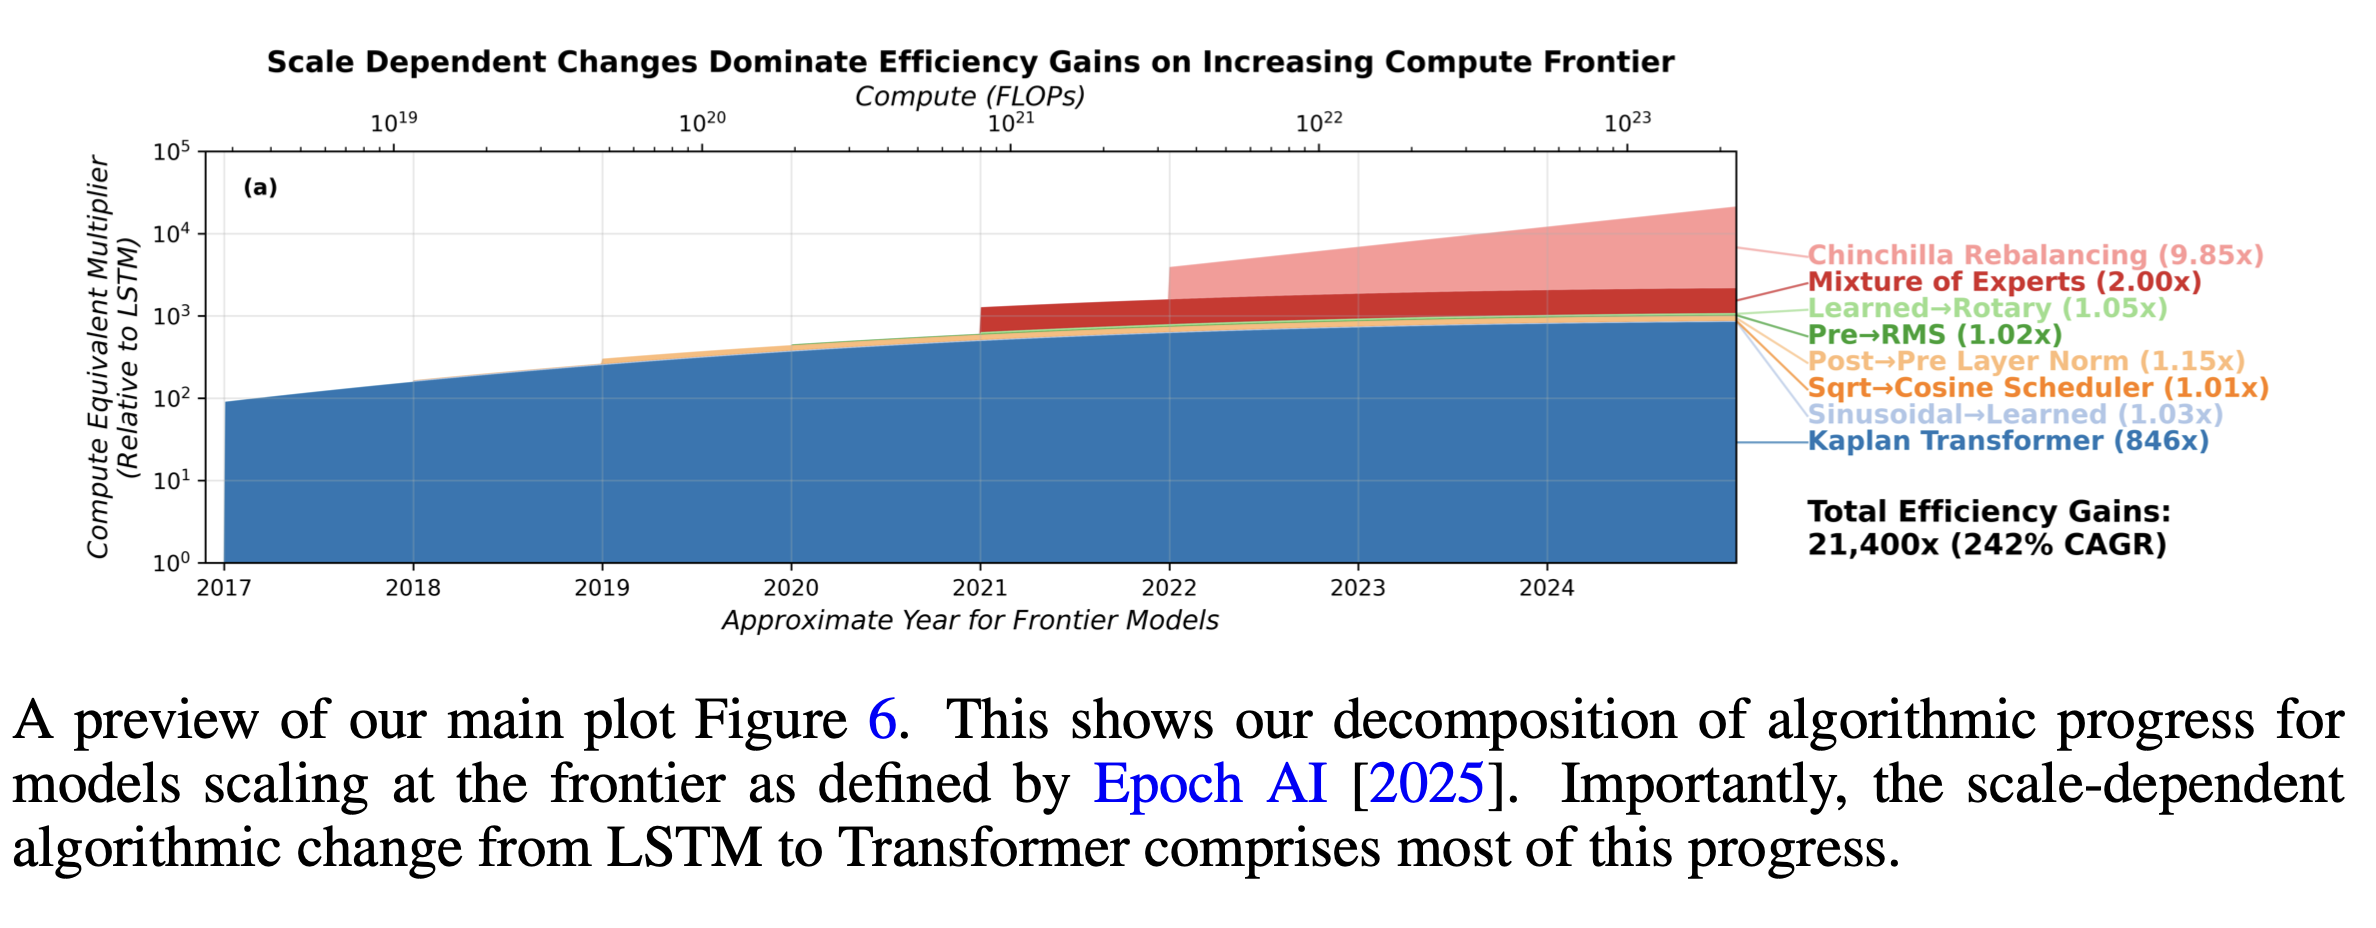
\includegraphics[keepaspectratio]{images/2026-02-25-05-18-41.png}}

}

\caption{Figure}

\end{figure}%

Estimates over 2012-2023:

\begin{itemize}
\tightlist
\item
  21,000X total (2.5X/year)
\item
  100X at small scale (1.5X/year), i.e.~if we hadn't scaled compute we'd
  only be increasing at 1.5X/year.
\end{itemize}
\item[Thompson, Ge, and Manso (2022) ``The Importance of (Exponentially
More) Computing Power'']
\begin{quote}
``we assemble direct quantitative evidence of the impact that computing
power has had on five domains: two computing bellwethers (Chess and Go),
and three economically important applications (weather prediction,
protein folding, and oil exploration). Computing power explains
49\%-94\% of the performance improvements in these domains.''
\end{quote}

{[}Not a direct estimate for LLM training efficiency, but useful
outside-view background for the broader compute-versus-algorithms
debate.{]}

\pandocbounded{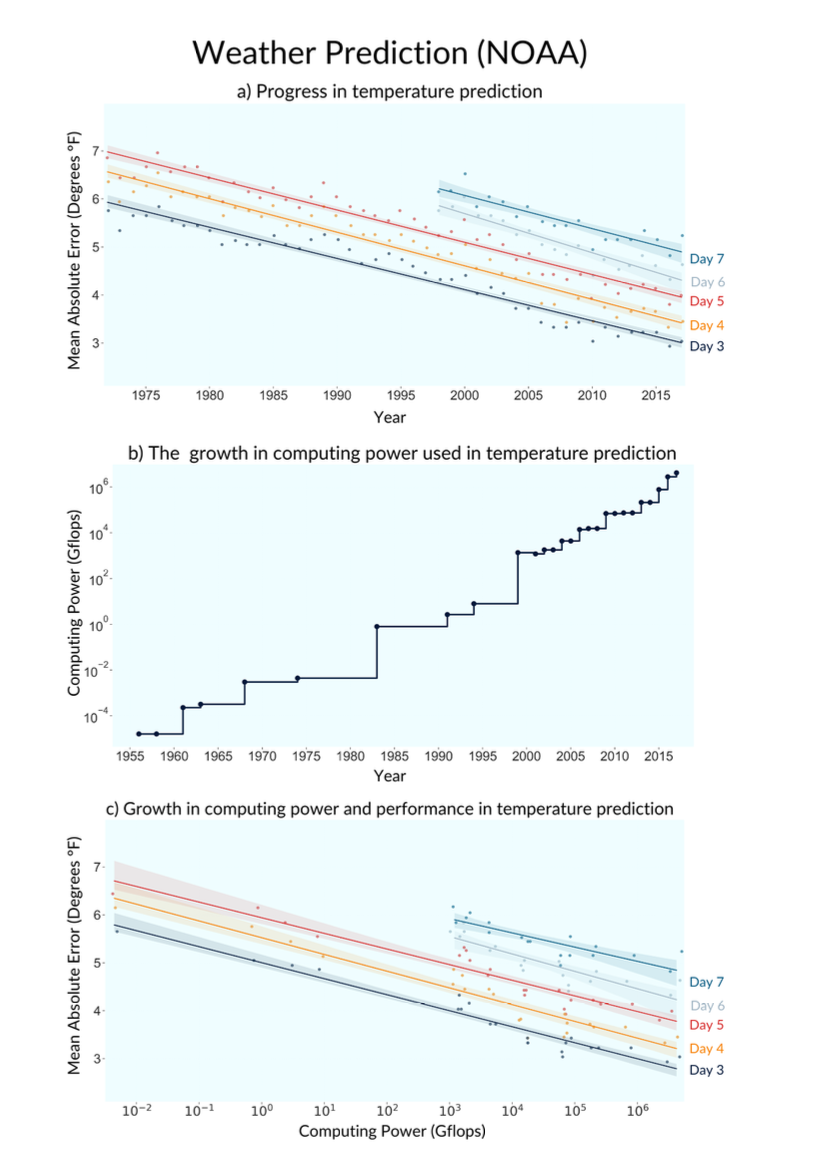
\includegraphics[keepaspectratio]{images/2023-11-03-17-44-38.png}}
\end{description}

\section{Literature Review on RSI
Models}\label{literature-review-on-rsi-models}

We want to answer these questions:

\begin{enumerate}
\def\labelenumi{\arabic{enumi}.}
\tightlist
\item
  Based on history of AI R\&D, what's a reasonable estimate of how AI
  R\&D will change the future trajectory?
\item
  What is the best capability metric for estimating AI R\&D
  contribution?
\end{enumerate}

Basic argument:

\begin{enumerate}
\def\labelenumi{\arabic{enumi}.}
\tightlist
\item
  Say algorithmic efficiency has been growing at 5X/year, so we can get
  the same intelligence for 5X lower cost.
\item
  We are starting to see glimmers of AI contributing to R\&D, \& want to
  predict how this will change the system.
\item
  Some alternatives in how to model this:

  \begin{itemize}
  \item
    \textbf{Accelerant.} Suppose a certain level of AI can speed up a
    human researcher by a certain proportion, \(\lambda\). This feedback
    loop should accelerate AI development, but it's sensitive to how
    strong this connection is.
  \item
    \textbf{Perfect substitutes.} Suppose AI can do entirely autonomous
    research, i.e.~it's a perfect substitute for a human. Then we are
    only constrained on the cost of AI compute. Unless the cost is very
    high, this implies a massive acceleration in AI progress,
    constrained only by (a) experiment bottlenecks; (b) a ceiling to AI
    progress.
  \item
    \textbf{Imperfect substitutes.}
  \end{itemize}
\item
  Endogenous growth setup: (1) diminishing returns to R\&D about 1/2;
  (2) increasing returns to knowledge about 1/2; these balance and get
  balanced growth.
\item
  Now we add link back from algorithms to R\&D, but very little guidance
  on how to calibrate it.
\end{enumerate}

Capability metrics:

\begin{enumerate}
\def\labelenumi{\arabic{enumi}.}
\tightlist
\item
  Human researcher uplift.
\item
  Ability to push forward the frontier.
\end{enumerate}

Wrinkles:

\begin{enumerate}
\def\labelenumi{\arabic{enumi}.}
\tightlist
\item
  Estimating algorithmic progress.
\item
  Scale-dependent algorithmic progress.
\item
  Bottlenecks on experiment compute.
\item
  Shape of the landscape.
\item
  Adding capital.
\end{enumerate}

Ajeya's questions:

\begin{enumerate}
\def\labelenumi{\arabic{enumi}.}
\tightlist
\item
  When will we have automated AI R\&D?

  \begin{itemize}
  \tightlist
  \item
    Answer: we already have automated R\&D.
  \end{itemize}
\item
  When we have automated AI R\&D, will this trigger super-exponential
  growth?
\end{enumerate}

Core model:

\[\begin{aligned}
    \utt{\dot{A}}{algorithmic}{progress}
        &=\utt{R^{\gamma}}{new}{research}
            {\utt{A^{1-\beta}}{algorithms}{}}
        && \text{(progress)}\\
    R&=A^{\kappa}
        && \text{}\\
    \dot{A}&=A^{1-\beta+\kappa}\\
\end{aligned}
\]

\begin{longtable}[]{@{}
  >{\raggedright\arraybackslash}p{(\linewidth - 4\tabcolsep) * \real{0.3068}}
  >{\raggedright\arraybackslash}p{(\linewidth - 4\tabcolsep) * \real{0.4904}}
  >{\raggedright\arraybackslash}p{(\linewidth - 4\tabcolsep) * \real{0.2027}}@{}}
\toprule\noalign{}
\begin{minipage}[b]{\linewidth}\raggedright
Model
\end{minipage} & \begin{minipage}[b]{\linewidth}\raggedright
Summary
\end{minipage} & \begin{minipage}[b]{\linewidth}\raggedright
\(r\) used / reported
\end{minipage} \\
\midrule\noalign{}
\endhead
\bottomrule\noalign{}
\endlastfoot
Charles I. Jones (1995) ``R\&D-Based Models of Economic Growth.'' &
Standard endogenous growth model: (1) diminishing returns to R\&D; (2)
positive spillovers from knowledge. & Defines the \(r=\lambda/\beta\)
object, but no numeric calibration here. \\
Aghion, Jones, and Jones (2019) ``Artificial Intelligence and Economic
Growth'' & They first model automation of goods tasks, then extend the
same task-based setup to research tasks; in the strong-form limit, AI
replaces people in idea production. & No standalone \(r\) calibration;
emphasis is on task shares and \(\phi\). \\
Davidson (2021) ``Could Advanced AI Drive Explosive Economic Growth'' &
The simplest model is where an AI robot perfectly substitutes for a
worker, \& then model the quantity increase of AI workers. & No single
\(r\); imports low-\(\beta\) software/hardware benchmarks via
\(\phi\). \\
Erdil et al. (2025) ``GATE: An Integrated Assessment Model for AI
Automation'' & They model both which tasks AI can do, and the quantity
of digital workers. & No single Jones-style \(r\) in this summary. \\
Davidson et al. (2026) ``When Does Automating AI Research Produce
Explosive Growth?'' & Partial automation of research tasks in a
networked multi-sector R\&D system; goods-task automation is also
present in the calibrated economy. They include cross-sector spillovers.
& Software \(r_S \sim 1\), hardware \(r_H=5\), aggregate innovation
\(r_A=0.32\). \\
B. F. Jones (2025) ``Artificial Intelligence in Research and
Development'' & AI progress causes both (1) a larger share of tasks to
be automated; (2) cost to drop for already-automated tasks. Task
bottlenecks determine the net impact. & No single numeric \(r\) in this
summary. \\
Kokotajlo et al. (2025) ``AI Futures Model: Dec 2025 Update'' &
Stagewise automation of AI R\&D: coding first, then research taste /
direction-setting; eventual full automation at SAR. & No explicit
Jones-style \(r\) calibration. \\
Eth and Davidson (2025) & Focuses directly on whether current software
R\&D has \(r>1\), rather than estimating \(\beta\) separately. & Argues
current software research may have \(r>1\). \\
Kwa (2026) ``Research Note: A Simpler AI Timelines Model Predicts 99\%
AI r\&d Automation in \textasciitilde2032'' & A simplification of
Kokotajlo et al. (2025), AI automates a fraction of tasks asymptotically
approaching 1, assume no substitutability between tasks. & No explicit
\(r\); assumes \(\beta \in [0.3,1]\). \\
& & \\
\end{longtable}

\begin{longtable}[]{@{}
  >{\raggedright\arraybackslash}p{(\linewidth - 4\tabcolsep) * \real{0.0983}}
  >{\raggedright\arraybackslash}p{(\linewidth - 4\tabcolsep) * \real{0.4301}}
  >{\raggedright\arraybackslash}p{(\linewidth - 4\tabcolsep) * \real{0.4716}}@{}}
\toprule\noalign{}
\begin{minipage}[b]{\linewidth}\raggedright
Mechanism
\end{minipage} & \begin{minipage}[b]{\linewidth}\raggedright
Examples
\end{minipage} & \begin{minipage}[b]{\linewidth}\raggedright
Comment
\end{minipage} \\
\midrule\noalign{}
\endhead
\bottomrule\noalign{}
\endlastfoot
\textbf{AI replaces R\&D workers} & Davidson (2021); late-stage AI
Futures; strong-form Aghion et al. & AI is effectively a
researcher/worker replacement, not just a helper on some tasks. \\
\textbf{AI automates a subset of general tasks} & Aghion et al.~(goods
side); GATE; parts of Davidson et al. & This is the
macro/task-automation framing: AI gradually expands over the
economy-wide task space. \\
\textbf{AI automates a subset of R\&D tasks} & Aghion et al.~(ideas
side); Davidson et al.; Ben Jones; AI Futures; Kwa & This is the most
common recent takeoff / AI-growth mechanism. \\
\textbf{AI increases productivity of R\&D workers} & Ben Jones
(fixed-task productivity gains); Besiroglu, Emery-Xu \& Thompson (2024);
early-stage AI Futures coding automation & This is the complementarity /
uplift box, where AI raises progress per dollar or per researcher
without immediately replacing everybody. \\
\textbf{AI replaces low-quality R\&D workers first} & \textbf{No clean
formal model among these}; closest is AI Futures' top-vs-median
milestone language & I would leave this as ``not really modeled yet''
rather than force one of these papers into the box. AI Futures comes
closest rhetorically, but it is not a true heterogeneous-worker
replacement model. ({[}AI Futures{]}{[}4{]}) \\
\textbf{Other mechanisms} & AI improves research taste (AI Futures);
increases digital-worker supply per automated task (GATE); raises
cross-sector spillovers (Davidson et al.); raises R\&D capital intensity
(Besiroglu et al.) & These are important because they are not just
``more tasks automated''; they change the mapping from capability to
research output. ({[}AI Futures{]}{[}4{]}) \\
\end{longtable}

\subsection{Charles I. Jones (1995) ``R\&D-Based Models of Economic
Growth''}\label{jones1995rd-rd-based-models-of-economic-growth}

I'll use the notation from Charles I. Jones (2022): \[\begin{aligned}
    Y_t &= A_t^\sigma L_{yt} 
        && \text{(final good)} \\
    \frac{\dot{A_t}}{A_t} &= R_t^\lambda A_t^{-\beta}
        && \text{(ideas)} \\
    R_t+L_{yt} &= L_t
        && \text{(resource constraint)} \\
    L_t &= L_0 e^{nt}
        && \text{(population growth)} \\
    R_t &= \bar{s}L_t
        && \text{(allocation)}
\end{aligned}
\]

Balanced-growth implications: \[\begin{aligned}
    g_A &= \frac{\lambda}{\beta}n \\
    g_y &= \sigma g_A = \frac{\lambda\sigma}{\beta}n = \gamma n
\end{aligned}
\]

Parameters:

\begin{longtable}[]{@{}
  >{\centering\arraybackslash}p{(\linewidth - 2\tabcolsep) * \real{0.2455}}
  >{\raggedright\arraybackslash}p{(\linewidth - 2\tabcolsep) * \real{0.7545}}@{}}
\toprule\noalign{}
\endhead
\bottomrule\noalign{}
\endlastfoot
\(\beta \approx 3\) & how fast proportional improvements are getting
harder to find. Jones writes that aggregate data are roughly consistent
with \(\beta \approx 3\) if \(\lambda = 1\). \\
\(\lambda \approx 1\) & elasticity of idea production with respect to
research effort. \(\lambda = 1\) means no duplication effect;
\(\lambda < 1\) allows duplication/congestion. \\
\(\sigma > 0\) & how strongly nonrival ideas raise final output; this is
the degree of increasing returns in goods production. He doesn't
separately calibrate. \\
\(\gamma \equiv \frac{\lambda\sigma}{\beta} \approx 1/3\) & the overall
degree of increasing returns in this simple semi-endogenous setup. Jones
says \(\gamma = 1/3\) is consistent with data when research intensity
has been rising. \\
\end{longtable}

\textbf{Visually:}

\begin{enumerate}
\def\labelenumi{\arabic{enumi}.}
\item
  Basic model with research effort but no knowledge term. If \(R\) is
  constant, then \(\dot{A}\) is constant, so \(A\) rises linearly and
  the growth rate \(g_A = \dot{A}/A\) declines toward zero:
  \[\begin{gathered}
   \dot{A}=R^\lambda\\
   \xymatrix{*++[F]{R\&D} \ar[r]|(0.4)\lambda & *++[F]{\Delta knowledge}\ar[r] & *++[F]{knowledge}}
   \end{gathered}
   \]
\item
  Add the knowledge term: \[\begin{gathered}
   \dot{A}=R^\lambda A^{1-\beta}\\
   \xymatrix{*++[F]{R\&D} \ar[r]|(0.4)\lambda & *++[F]{\Delta knowledge}\ar[r] & *++[F]{knowledge}\ar@/^2em/[l]|{1-\beta}}
   \end{gathered}
   \]

  Then \(g_A = \frac{\dot{A}}{A} = R^\lambda A^{-\beta}.\)

  So if \(R\) is constant, \(g_A\) declines as \(A\) rises.\footnote{Charles
    I. Jones (1995) introduced diminishing returns to knowledge, whereas
    Romer (1990) had assumed no diminishing returns to knowledge,
    \(\beta=0\).} If \(R\) grows at rate \(g_R\) along a balanced growth
  path, then \(g_A = \frac{\lambda}{\beta}g_R.\)
\item
  Recursive self-improvement, where knowledge directly raises research
  input: \[\begin{gathered}
   R=A^\kappa\\
   \dot{A}=(A^\kappa)^\lambda A^{1-\beta}=A^{\lambda\kappa+1-\beta}\\
   \xymatrix{*++[F]{R\&D} \ar[r]|(0.4)\lambda & *++[F]{\Delta knowledge}\ar[r] & *++[F]{knowledge}\ar@/^2em/[l]|{1-\beta}\ar@/^4em/[ll]|\kappa}
   \end{gathered}
   \]

  This yields:

  \begin{itemize}
  \tightlist
  \item
    if \(\lambda\kappa < \beta\), growth slows over time;
  \item
    if \(\lambda\kappa = \beta\), you get constant exponential growth;
  \item
    if \(\lambda\kappa > \beta\), the model implies a finite-time
    singularity.
  \end{itemize}
\end{enumerate}

\subsection{Aghion, Jones, and Jones (2019)}\label{aghion2019artificial}

Setup:

\[\begin{aligned}
         Y_t &= A_t^{\sigma} K_t^{\alpha} L^{1-\alpha} \\
         \dot A_t &= K_t^{\beta} S^{\lambda} A_t^{\phi}
      \end{aligned}
\]

Implications / thresholds:

\begin{itemize}
\tightlist
\item
  In this notation, \(\alpha\) is the capital exponent in goods
  production and \(\beta\) is the capital exponent in idea production;
  the ``ideas getting harder to find'' term is \(\phi < 1\), not Jones's
  \(\beta\).
\item
  In the paper's task-automation framing, more automation raises the
  role of capital in both sectors, which can raise the long-run growth
  rate by making research effort more accumulable.
\item
  The paper distinguishes Type I growth explosions, where growth rates
  rise without bound but remain finite at each date, from Type II
  explosions, where output becomes infinite in finite time.
\item
  Type I condition in their examples: full automation of goods
  production. Once all goods tasks are automated, the goods sector
  becomes an AK-style economy, \(Y_t = A_tK_t\), and with ongoing
  technological progress the growth rate \(g_Y = g + sA_t\) rises
  without bound.
\item
  Type II condition in their Example 2: full automation of ideas
  production. In their one-dimensional analogue this becomes
  \(\dot{A}_t = A_t^{1+\phi}\), so explosive growth requires \(\phi>0\).
\item
  Type II can also arise without full automation in their Cobb-Douglas
  Example 3, where a key ``constant returns to accumulable factors''
  parameter exceeds one.
\end{itemize}

\begin{longtable}[]{@{}
  >{\raggedright\arraybackslash}p{(\linewidth - 2\tabcolsep) * \real{0.0667}}
  >{\raggedright\arraybackslash}p{(\linewidth - 2\tabcolsep) * \real{0.9333}}@{}}
\toprule\noalign{}
\endhead
\bottomrule\noalign{}
\endlastfoot
\(\alpha\) & capital exponent in goods production. \\
\(\beta\) & capital exponent in idea production. \\
\(\lambda\) & elasticity of idea production with respect to research
labor. \\
\(\phi\) & standing-on-shoulders term in the paper's notation, with
Jones-style harder-to-find parameter
\(\beta_{\text{Jones}} = 1-\phi\). \\
\(\sigma\) & role of nonrival ideas in final output. \\
& \\
\end{longtable}

\subsection{Davidson (2021)}\label{davidson2021could}

Davidson writes idea production in \(\phi\)-notation rather than Jones
\(\beta\)-notation, so the mapping is \(\beta = 1-\phi\).

\begin{itemize}
\tightlist
\item
  Aggregate innovation: \(\phi=-2.1 \Rightarrow \beta \approx 3.1\).
\item
  Hardware: \(\phi=0.8 \Rightarrow \beta \approx 0.2\).
\item
  ML software: \(\phi=0.85 \Rightarrow \beta \approx 0.15\).
\end{itemize}

This is one of the main routes by which very low software \(\beta\)
enters AI-takeoff discussions. But it is best read as importing earlier
subsector estimates in \(\phi\)-notation, not as a fresh direct estimate
of frontier-AI-lab \(\beta\).

\subsection{Erdil and Besiroglu (2024) ``Explosive growth from AI
automation: A review of the
arguments''}\label{erdil2024explosive-explosive-growth-from-ai-automation-a-review-of-the-arguments}

\begin{quote}
``Bloom et al.~2020, which provides us perhaps with the best estimates
of the extent to which ideas get ``harder to find'', estimates that λ/ϕ
≈ 0.32 for total factor productivity in the US economy. Based on this,
we find that hyperbolic growth occurs with values of β as low as 1 −
0.32 = 0.68. Hence, hyperbolic growth with AI is predicted by R\&D-based
growth models even if we do not strictly accept the conclusion of the
replication argument that β = 1. This point, that avoiding increasing
returns to scale is difficult to avoid even when ideas get ``harder to
find'' over time, has been noted elsewhere, notably by Davidson 2021.
Indeed, this outcome is consistent with fairly conservative assumption
on there being decreasing returns on inputs to final goods production.''
\end{quote}

\subsection{Erdil, Besiroglu, and Ho (2024) ``Estimating Idea
Production: A Methodological
Survey''}\label{erdil2024estimating-estimating-idea-production-a-methodological-survey}

\[\begin{aligned}
    Y &= AK^\alpha \\
    \dot{K} &\propto Y && \text{(constant savings rate)}\\
    \dot{A}/A &\propto A^{-\beta}K^\lambda && \text{(productivity growth)}
\end{aligned}
\]

Parameters:

\begin{longtable}[]{@{}
  >{\raggedright\arraybackslash}p{(\linewidth - 2\tabcolsep) * \real{0.1318}}
  >{\raggedright\arraybackslash}p{(\linewidth - 2\tabcolsep) * \real{0.8682}}@{}}
\toprule\noalign{}
\endhead
\bottomrule\noalign{}
\endlastfoot
\(\alpha\) & capital elasticity in final output. \\
\(\lambda\) & elasticity of productivity growth with respect to R\&D
input. \\
\(\beta\) & ideas-get-harder-to-find parameter. \\
\(r=\lambda/\beta\simeq 1\) & the object the paper argues is usually
identified more robustly than either numerator or denominator on its
own. \\
& \\
\end{longtable}

Implications / thresholds:

\begin{itemize}
\tightlist
\item
  The paper's main methodological lesson is that much of this literature
  identifies \(r=\lambda/\beta\) more cleanly than it identifies
  \(\beta\) itself.
\item
  In their simple growth setup, you get steady-state growth if and only
  if \(\lambda/\beta+\alpha=1\).
\item
  You get hyperbolic growth if \(\lambda/\beta+\alpha>1\).
\end{itemize}

In the best high-frequency software case study they discuss, Stockfish,
the central estimate is \(r \approx 0.83\) with standard error \(0.15\).
For sparser domains, their Bayesian posterior medians are:

\begin{longtable}[]{@{}
  >{\raggedright\arraybackslash}p{(\linewidth - 8\tabcolsep) * \real{0.2743}}
  >{\raggedright\arraybackslash}p{(\linewidth - 8\tabcolsep) * \real{0.1150}}
  >{\raggedright\arraybackslash}p{(\linewidth - 8\tabcolsep) * \real{0.2124}}
  >{\raggedright\arraybackslash}p{(\linewidth - 8\tabcolsep) * \real{0.1947}}
  >{\raggedright\arraybackslash}p{(\linewidth - 8\tabcolsep) * \real{0.2035}}@{}}
\toprule\noalign{}
\begin{minipage}[b]{\linewidth}\raggedright
domain
\end{minipage} & \begin{minipage}[b]{\linewidth}\raggedright
doubling time
\end{minipage} & \begin{minipage}[b]{\linewidth}\raggedright
median \(r=\lambda/\beta\)
\end{minipage} & \begin{minipage}[b]{\linewidth}\raggedright
β
\end{minipage} & \begin{minipage}[b]{\linewidth}\raggedright
λ
\end{minipage} \\
\midrule\noalign{}
\endhead
\bottomrule\noalign{}
\endlastfoot
Stockfish & & 0.83 & & \\
Computer vision, 2012-2022 & 9 months & 1.44 & 0.985 (0.224 to 4.050) &
1.410 (0.290 to 6.021) \\
RL sample efficiency, 2015-2019 & 11 months & 1.58 & 1.023 (0.212 to
3.914) & 1.482 (0.266 to 6.650) \\
SAT solvers, 1997-2018 & 2 years & 3.54 & 0.648 (0.139 to 2.891) & 2.143
(0.387 to 11.312) \\
Linear programming, 1998-2018 & 6 years & 1.08 & 1.290 (0.254 to 4.953)
& 1.259 (0.222 to 5.772) \\
\end{longtable}

\subsection{Kokotajlo et al. (2025) AI futures
model}\label{kokotajlo2025aifuturesmodel-ai-futures-model}

More complicated!

\subsection{Ho and Whitfill (2025) ``The software intelligence explosion
debate needs
experiments''}\label{ho2025explosionexperiments-the-software-intelligence-explosion-debate-needs-experiments}

Equations:

\[\dot{A} = A^{1-\beta}F(L,K)^\lambda\]

If research automation makes effective research input proportional to
algorithmic progress itself, so that \(F(L,K)\propto cA\), then

\[\dot{A} \propto A^{\lambda+1-\beta}.\]

Implications / thresholds:

\begin{itemize}
\tightlist
\item
  In this setup, the key threshold is \(r\equiv\frac{\lambda}{\beta}\).
\item
  You get explosive growth if \(r>1\).
\item
  In their domain-level estimates, the NLP / language-model proxy is the
  strongest case for \(r>1\), but the uncertainty intervals are still
  very wide.
\item
  In their OpenAI 2022-2025 back-of-the-envelope exercise, the central
  estimate is \(r \approx 0.96\), and under a Cobb-Douglas bottleneck
  story the relevant object becomes \((1-\epsilon_K)\lambda/\beta\),
  which pushes the effective value further below \(1\).
\end{itemize}

This is the cleanest direct \(\beta\) estimation exercise I have found
that is actually about AI-ish domains rather than aggregate innovation
or imported hardware benchmarks. The key caveat is that the intervals
are extremely wide.

\begin{longtable}[]{@{}
  >{\raggedright\arraybackslash}p{(\linewidth - 8\tabcolsep) * \real{0.1259}}
  >{\raggedright\arraybackslash}p{(\linewidth - 8\tabcolsep) * \real{0.2074}}
  >{\raggedright\arraybackslash}p{(\linewidth - 8\tabcolsep) * \real{0.1778}}
  >{\raggedright\arraybackslash}p{(\linewidth - 8\tabcolsep) * \real{0.2444}}
  >{\raggedright\arraybackslash}p{(\linewidth - 8\tabcolsep) * \real{0.2444}}@{}}
\toprule\noalign{}
\begin{minipage}[b]{\linewidth}\raggedright
\end{minipage} & \begin{minipage}[b]{\linewidth}\raggedright
computer vision
\end{minipage} & \begin{minipage}[b]{\linewidth}\raggedright
reinforcement learning
\end{minipage} & \begin{minipage}[b]{\linewidth}\raggedright
natural language processing proxy
\end{minipage} & \begin{minipage}[b]{\linewidth}\raggedright
OpenAI 2022-2025 back-of-envelope
\end{minipage} \\
\midrule\noalign{}
\endhead
\bottomrule\noalign{}
\endlastfoot
\(\beta\) & 1.302 (90\% CrI 0.269-5.571) & 1.299 (0.241-5.581) & 1.586
(0.322-7.148) & not separately identified \\
\(r=\lambda/\beta\) & 1.262 & 1.201 & 1.892 & about 0.96 \\
\end{longtable}

\begin{longtable}[]{@{}
  >{\raggedright\arraybackslash}p{(\linewidth - 2\tabcolsep) * \real{0.1008}}
  >{\raggedright\arraybackslash}p{(\linewidth - 2\tabcolsep) * \real{0.8992}}@{}}
\toprule\noalign{}
\endhead
\bottomrule\noalign{}
\endlastfoot
\(\beta\) & the ideas-get-harder-to-find parameter for AI software. \\
\(\lambda\) & the elasticity of progress with respect to effective
research input. \\
\(\epsilon_K\) & the elasticity of research input with respect to
experiment compute in the Cobb-Douglas bottleneck variant. \\
\end{longtable}

Their proxies for software quality are based on measures of training
compute efficiency. They note that if \(A\) is inference compute
efficiency, the augmentation equation holds exactly; if \(A\) is
training compute efficiency, it requires an additional linearity
assumption connecting training efficiency to effective AI researchers.

\subsection{Erdil and Barnett (2025) ``Most AI value will come from
broad automation, not from
R\&D''}\label{erdil2025automatingrd-most-ai-value-will-come-from-broad-automation-not-from-rd}

They give arguments for why AI R\&D will be bottlenecked by experiment
compute:

\begin{quote}
``By default, a software-only or software-biased singularity should be
treated as an unlikely outcome rather than a likely one.''
\end{quote}

\begin{quote}
``If the two inputs are indeed complementary, any software-driven
acceleration could only last until we become bottlenecked on compute and
end up having to do the physical work of obtaining more GPUs in order to
run more experiments.''
\end{quote}

\begin{quote}
``Just as one example, Oberfield and Raval (2014) estimate that the
elasticity of substitution between labor and capital in the US
manufacturing sector is 0.7, and this is already strong enough for any
``software-only singularity'' to fizzle out after less than an order of
magnitude of improvement in efficiency.''
\end{quote}

\subsection{Eth and Davidson (2025)}\label{eth2025willairdautomati}

\begin{quote}
``More specifically, r gives the number of times software doubles for
each time the cumulative work on software R\&D doubles \ldots{} There
are a few reasons to think that r is currently above 1:''
\end{quote}

Implications / thresholds:

\begin{itemize}
\tightlist
\item
  The paper's question is whether current software R\&D has \(r>1\),
  since that is the relevant threshold for a software intelligence
  explosion in the simplest Jones-style setup.
\item
  The nearby empirical anchors are also mostly estimates of \(r\): in
  the best high-frequency software case study, Stockfish, the central
  estimate is \(r \approx 0.83\) with standard error \(0.15\); in
  sparser software domains the Bayesian posterior medians are about
  \(1.44\) for computer vision, \(1.58\) for RL sample efficiency,
  \(3.54\) for SAT, and \(1.08\) for linear programming Erdil,
  Besiroglu, and Ho (2024).
\end{itemize}

Those numbers matter for whether recursive improvement crosses the
critical threshold, but they do not separately identify \(\beta\) unless
we also know \(\lambda\).

\subsection{Davidson and Houlden
(2025)}\label{davidson2025howquickandbigwo}

\[
\begin{aligned}
\dot S(L, C) &= a [R(L, C)]^\lambda S^{1-\beta} && \text{(Software L.O.M.)} \\
R(L, C) &= (bL)^\alpha (cC)^{1-\alpha} && \text{(Research Input)} \\
L &= dS && \text{(Cognitive Labour)}
\end{aligned}
\]

Parameters:

\begin{longtable}[]{@{}
  >{\raggedright\arraybackslash}p{(\linewidth - 2\tabcolsep) * \real{0.0659}}
  >{\raggedright\arraybackslash}p{(\linewidth - 2\tabcolsep) * \real{0.9341}}@{}}
\toprule\noalign{}
\endhead
\bottomrule\noalign{}
\endlastfoot
\(S\) & is the level of AI software. \\
\(L\) & is the cognitive labour used for improving software. \\
\(C\) & is compute for experiments, assumed to be constant. \\
\(\lambda\) & captures ``stepping on toes,'' whereby there are
diminishing returns to applying more research effort in parallel (``nine
women can't make a baby in a month''). \\
\(\beta \approx 0.25\) & captures the idea that software improvements
get harder to find as software improves. \\
\(\alpha\) & captures the diminishing returns of cognitive labour in
improving software. \\
r=\lambda\alpha/\beta\approx 1.2 & \\
\end{longtable}

Implications / thresholds:

\begin{itemize}
\tightlist
\item
  The key threshold is \(r=\lambda\alpha/\beta\).
\item
  The paper calibrates primarily in terms of \(p\) and \(r\), not by
  directly estimating \(\beta\).
\item
  Their reported medians are \(p=0.3\) and \(r=1.2\), and one
  representative decomposition is \(\alpha=0.5\), \(\lambda=0.6\), and
  \(\beta=0.25\).
\end{itemize}

\subsection{Kokotajlo et al. (2025) ``AI Futures Model: Dec 2025
Update''}\label{kokotajlo2025aifuturesmodel-ai-futures-model-dec-2025-update}

\begin{quote}
``Davidson and Houlden focuses primarily on trends of how much more
efficiently AIs have been able to achieve the same performance when
determining whether there will be an SIE. Meanwhile, we focus on
estimates of the quality of AIs' research taste, i.e.~how good the AI is
at choosing research directions, selecting and interpreting experiments,
etc. We think that focusing on research taste quality is a more useful
lens from which to view a potential SIE. If there's an SIE we expect
that it will primarily be driven by improvements in research taste.''
\end{quote}

Superhuman AI Researcher = ``An AI system that can do the job of the
best human AI researcher but 30x faster and with 30x more agents, as
defined above in the superhuman coder milestone. It must have enough
diversity of expertise to on average do the same for other top
researchers with complementary skills.''

\subsection{Davidson et al. (2026) ``When Does Automating Research
Produce Explosive
Growth?''}\label{davidson2026automatingairesearch-when-does-automating-research-produce-explosive-growth}

Summary: once you automate a sufficient number of tasks (i.e.~do them
with capital) then this will kick-off an intelligence explosion.

\[\begin{aligned}
    \dot{S}(L,C) &= a [R(L,C)]^\lambda S^{1-\beta_S} && \text{(software law of motion)} \\
    R(L,C) &= (bL)^\alpha (cC)^{1-\alpha} && \text{(Research Input)} \\
    L &= dS && \text{(Cognitive Labour)}
\end{aligned}
\]

Parameters:

\begin{longtable}[]{@{}
  >{\raggedright\arraybackslash}p{(\linewidth - 2\tabcolsep) * \real{0.1667}}
  >{\raggedright\arraybackslash}p{(\linewidth - 2\tabcolsep) * \real{0.8333}}@{}}
\toprule\noalign{}
\endhead
\bottomrule\noalign{}
\endlastfoot
\(\beta_S \approx 1\) & software ideas-get-harder-to-find parameter,
citing Ho and Whitfill (2025) and Erdil, Besiroglu, and Ho (2024). \\
\(\beta_H \approx 0.2\) & hardware ideas-get-harder-to-find
parameter. \\
\(\beta_A \approx 3.1\) & aggregate innovation ideas-get-harder-to-find
parameter. \\
\(\alpha\) & labor elasticity in the research-input aggregator. \\
\(\lambda\) & stepping-on-toes / parallelization parameter. \\
\(r_S\approx 1\) & \\
\(r_H\approx 5\) & \\
\(r_A\approx 0.32\) & \\
\end{longtable}

Critical condition for explosive growth:

\[
    \utt{f_Y}{share output}{tasks automated} + 
    \utt{f_S}{share software}{tasks automated}\frac{1}{\beta_S} + 
    \utt{f_H}{share hardware}{tasks automated}\frac{1}{\beta_H} + 
    \utt{f_A}{share innovation}{tasks automated}\frac{1}{\alpha}\frac{1}{\beta_A}
    >1
\]

\begin{itemize}
\tightlist
\item
  Basic model:

  \begin{itemize}
  \tightlist
  \item
    If \(\dot{S}_t=S_t^{1-\beta}\), so you get explosion if \(\beta<0\),
    steady-state growth if \(\beta=0\), and gradual slowing if
    \(\beta>1\).
  \item
    Now if you start automating inputs, the effective exponent gradually
    gets higher.
  \end{itemize}
\item
  Multi-sector version.

  \begin{itemize}
  \tightlist
  \item
    You gradually automate some of the things, so they can be done with
    capital.
  \item
    You have spillovers between different processes.
  \end{itemize}
\end{itemize}

Implications / thresholds:

\begin{itemize}
\tightlist
\item
  In the one-sector software model, the key threshold is
  \(r = \lambda\alpha/\beta_S\).
\item
  In the multi-sector model, explosive growth can arise from the
  combined automation of goods production, software R\&D, hardware
  progress, and aggregate innovation, even when no single channel is
  decisive on its own.
\end{itemize}

\subsection{Kwa (2026) tkwa~
model}\label{kwa2026simpleraitimelines-tkwa-model}

Equations:

\[
\begin{aligned}
   S'(t) &= R(t) S^{1 - \beta} = \left(\frac L {1-f}\right)^\alpha C^\zeta S^{1 - \beta}
    && \text{(accumulation of software ideas)}\\
   f(t) &= \sigma(v(\log C(t)S(t) - \log E_{hac})) 
    && \text{(automation of tasks)}
\end{aligned}
\]

Automating a fraction \(f\) of R\&D tasks multiplies effective R\&D
labor by \(1/(1-f)\) (i.e.~tasks are perfect complements).

\[\begin{aligned}
   \dot{S}  &= L^\alpha C^\gamma S^{1-\beta} \\
\end{aligned}
\]

Parameters:

\begin{longtable}[]{@{}
  >{\raggedright\arraybackslash}p{(\linewidth - 2\tabcolsep) * \real{0.1954}}
  >{\raggedright\arraybackslash}p{(\linewidth - 2\tabcolsep) * \real{0.8046}}@{}}
\toprule\noalign{}
\endhead
\bottomrule\noalign{}
\endlastfoot
\(\beta\in [0.3,1]\) & software-difficulty exponent. \\
\(\alpha\) & not pinned down separately; together with \(\zeta\), Kwa
uses \(\alpha/(\alpha+\zeta)\in [0.12,0.35]\) and
\(\alpha+\zeta\in [0.8,1]\), implying roughly
\(\alpha\in [0.10,0.35]\). \\
\(\zeta\) & not pinned down separately; implied by the same calibration
above, roughly \(\zeta\in [0.52,0.88]\). \\
\(f(t)\) & fraction of R\&D tasks automated; Kwa sets current \(f\) in
Jan 2026 to lie in \([0.25,0.5]\). \\
\(v\) & automation velocity; Kwa uses \(1/v\in [1.5,4.2]\), so
\(v\in [0.24,0.67]\). \\
\(E_{hac}\) & effective compute level of the half-automated coder; not
directly estimated here, but defined as the point where automation
reaches 50\%. \\
\end{longtable}

Relevant notes on interpretation / sources:

\begin{quote}
``\(E_{hac}\) is the effective compute level of the half-automated
coder''
\end{quote}

\begin{quote}
``v is the automation velocity: S must increase by factor of e\^{}(1/v)
to get from 50\% to 73\% automation''
\end{quote}

\begin{quote}
``alpha/(alpha + zeta) is between 0.12 and 0.35 \ldots{} This range is
based on Yafah's (Epoch) recommendation to calibrate from lab spending
ratios of labor vs capital.''
\end{quote}


\includegraphics[width=13.92in,height=4.5in]{2025-09-13-recursive-self-improvement-explosion-optimization_files/figure-latex/mermaid-figure-1.png}


\includegraphics[width=8.73in,height=3.44in]{2025-09-13-recursive-self-improvement-explosion-optimization_files/figure-latex/mermaid-figure-2.png}

\subsection{David Rein (2025) model}\label{david-rein-2025-model}

The core idea: idea production depends on quality:

\[\begin{aligned}
    dA &= Q^q A^{1-\beta}
         && \text{(idea production depends on quality of cognitive labor)}\\
    Q &= cA
        && \text{(quality depends on ideas)}
\end{aligned}
\]

Parameters: \textbar{} \textbar{} \textbar{} \textbar{} -------
\textbar{}
-----------------------------------------------------------------------------------------------------------------------------
\textbar{} \textbar{} \(Q\) \textbar{} quality of cognitive labour,
measured in units of time horizon; this is our AI researcher (e.g.~Opus
4.5, GPT-5.2, Gemini 3). \textbar{} \textbar{} \(A\) \textbar{} current
level of algorithms, also measured in units of time horizon (e.g.~GPT-2,
GPT-3, Pythia, etc.). \textbar{} \textbar{} \(q\) \textbar{} elasticity
of idea production with respect to cognitive-labor quality. \textbar{}
\textbar{} \(\beta\) \textbar{} ideas-get-harder-to-find parameter.
\textbar{}

Implications / thresholds:

\begin{itemize}
\tightlist
\item
  The explosion condition is \(q > \beta\).
\end{itemize}

\href{https://docs.google.com/document/d/16Ugl7g3GL1Ao9-3UluRENp6e9UeEMAqhh5jgXDi3kjo/edit?tab=t.a5tu3xadb63o\#heading=h.ribcf6q6wbps}{source}

\phantomsection\label{refs}
\begin{CSLReferences}{1}{0}
\bibitem[\citeproctext]{ref-aghion2019artificial}
Aghion, Philippe, Benjamin F. Jones, and Charles I. Jones. 2019.
{``Artificial Intelligence and Economic Growth.''} In \emph{The
Economics of Artificial Intelligence: An Agenda}, edited by Ajay
Agrawal, Joshua Gans, and Avi Goldfarb, 237--90. Chicago: University of
Chicago Press. \url{https://doi.org/10.7208/9780226613475-011}.

\bibitem[\citeproctext]{ref-amodei2018aiandcompute}
Amodei, Dario, and Danny Hernandez. 2018. {``AI and Compute.''}
\url{https://openai.com/index/ai-and-compute/}.

\bibitem[\citeproctext]{ref-anthropic2025claude_work}
Anthropic. 2025. {``Claude at Work: How Anthropic Uses Claude Code
Internally.''}
\url{https://assets.anthropic.com/m/6cd21f7d4f82afcb/original/Claude-at-Work-Survey.pdf}.

\bibitem[\citeproctext]{ref-byrnes2026naturellmalgorithmicprogress}
Byrnes, Steven. 2026. {``The Nature of {LLM} Algorithmic Progress
(V2).''}
\url{https://www.lesswrong.com/posts/sGNFtWbXiLJg2hLzK/the-nature-of-llm-algorithmic-progress-v2}.

\bibitem[\citeproctext]{ref-davidson2021could}
Davidson, Tom. 2021. {``Could Advanced AI Drive Explosive Economic
Growth.''} \emph{Open Philanthropy} 25.
\url{https://www.openphilanthropy.org/research/could-advanced-ai-drive-explosive-economic-growth}.

\bibitem[\citeproctext]{ref-davidson2026automatingairesearch}
Davidson, Tom, Basil Halperin, Thomas Houlden, and Anton Korinek. 2026.
{``When Does Automating AI Research Produce Explosive Growth?''}
\url{https://www.basilhalperin.com/papers/shs.pdf}.

\bibitem[\citeproctext]{ref-davidson2025howquickandbigwo}
Davidson, Tom, and Tom Houlden. 2025. {``How Quick and Big Would a
Software Intelligence Explosion Be?''}
\url{https://www.forethought.org/research/how-quick-and-big-would-a-software-intelligence-explosion-be}.

\bibitem[\citeproctext]{ref-epoch2025computescaling}
Edelman, Yafah, and Anson Ho. 2025. {``Compute Scaling Will Slow down
Due to Increasing Lead Times.''}
\url{https://epoch.ai/gradient-updates/compute-scaling-will-slow-down-due-to-increasing-lead-times/}.

\bibitem[\citeproctext]{ref-efrati2025openaicomputingcostproblem}
Efrati, Amir, and Sri Muppidi. 2025.
\url{https://www.theinformation.com/articles/openais-350-billion-computing-cost-problem}.

\bibitem[\citeproctext]{ref-epoch2025trainingcomputefrontier}
Epoch AI. 2025a. {``Training Compute of Frontier AI Models Grows by 4-5x
Per Year.''}
\url{https://epoch.ai/blog/training-compute-of-frontier-ai-models-grows-by-4-5x-per-year}.

\bibitem[\citeproctext]{ref-EpochAIModels2025}
---------. 2025b. {``Data on AI Models.''}
\url{https://epoch.ai/data/ai-models/}.

\bibitem[\citeproctext]{ref-epoch2026computetrendpost2010}
---------. 2026a. {``The Training Compute of Notable AI Models Has Been
Doubling Roughly Every Six Months.''}
\url{https://epoch.ai/data-insights/compute-trend-post-2010}.

\bibitem[\citeproctext]{ref-EpochAITrends2026}
---------. 2026b. {``Trends in Artificial Intelligence.''}
\url{https://epoch.ai/trends}.

\bibitem[\citeproctext]{ref-erdil2025automatingrd}
Erdil, Ege, and Matthew Barnett. 2025. {``Most AI Value Will Come from
Broad Automation, Not from r\&d.''}
\url{https://epoch.ai/gradient-updates/most-ai-value-will-come-from-broad-automation-not-from-r-d}.

\bibitem[\citeproctext]{ref-erdil2024explosive}
Erdil, Ege, and Tamay Besiroglu. 2024. {``Explosive Growth from AI
Automation: A Review of the Arguments.''}
\url{https://arxiv.org/abs/2309.11690}.

\bibitem[\citeproctext]{ref-erdil2024estimating}
Erdil, Ege, Tamay Besiroglu, and Anson Ho. 2024. {``Estimating Idea
Production: A Methodological Survey,''} May.
\url{https://doi.org/10.2139/ssrn.4814445}.

\bibitem[\citeproctext]{ref-erdil2025gate}
Erdil, Ege, Andrei Potlogea, Tamay Besiroglu, Edu Roldan, Anson Ho,
Jaime Sevilla, Matthew Barnett, Matej Vrzla, and Robert Sandler. 2025.
{``GATE: An Integrated Assessment Model for AI Automation.''}
\emph{arXiv Preprint arXiv:2503.04941}.
\url{https://arxiv.org/pdf/2503.04941.pdf}.

\bibitem[\citeproctext]{ref-eth2025willairdautomati}
Eth, Daniel, and Tom Davidson. 2025. {``Will AI r\&d Automation Cause a
Software Intelligence Explosion?''}
\url{https://www.forethought.org/research/will-ai-r-and-d-automation-cause-a-software-intelligence-explosion}.

\bibitem[\citeproctext]{ref-gundlach2025algorithmicprogressai}
Gundlach, Hans, Alex Fogelson, Jayson Lynch, Ana Trisovic, Jonathan
Rosenfeld, Anmol Sandhu, and Neil Thompson. 2025. {``On the Origin of
Algorithmic Progress in AI.''} \url{https://arxiv.org/abs/2511.21622}.

\bibitem[\citeproctext]{ref-ho2026leastunderstooddriver}
Ho, Anson. 2026. {``The Least Understood Driver of AI Progress.''}
\url{https://epoch.ai/gradient-updates/the-least-understood-driver-of-ai-progress}.

\bibitem[\citeproctext]{ref-ho2024algorithmicprogresslm}
Ho, Anson, Tamay Besiroglu, Ege Erdil, David Owen, Robi Rahman, Zifan
Carl Guo, David Atkinson, Neil Thompson, and Jaime Sevilla. 2024.
{``Algorithmic Progress in Language Models.''}
\url{https://doi.org/10.48550/arXiv.2403.05812}.

\bibitem[\citeproctext]{ref-ho2025explosionexperiments}
Ho, Anson, and Parker Whitfill. 2025. {``The Software Intelligence
Explosion Debate Needs Experiments.''}
\url{https://epoch.ai/gradient-updates/the-software-intelligence-explosion-debate-needs-experiments}.

\bibitem[\citeproctext]{ref-jones2025aird}
Jones, Benjamin F. 2025. {``Artificial Intelligence in Research and
Development.''} NBER Working Paper 34312. National Bureau of Economic
Research. \url{https://doi.org/10.3386/w34312}.

\bibitem[\citeproctext]{ref-jones1995rd}
Jones, Charles I. 1995. {``R\&d-Based Models of Economic Growth.''}
\emph{Journal of Political Economy} 103 (4): 759--84.
https://doi.org/\url{https://doi.org/10.1086/262002}.

\bibitem[\citeproctext]{ref-jones2022semiendogenous}
Jones, Charles I. 2022. {``The Past and Future of Economic Growth: A
Semi-Endogenous Perspective.''} \emph{Annual Review of Economics} 14
(1): 125--52.
\url{https://doi.org/10.1146/annurev-economics-080521-012458}.

\bibitem[\citeproctext]{ref-kellerjordan2026moddednanogpt}
Jordan, Keller, and contributors. 2026. {``Modded-Nanogpt.''}
\url{https://github.com/KellerJordan/modded-nanogpt}.

\bibitem[\citeproctext]{ref-karpathy2024llmcdiscussion}
Karpathy, Andrej. 2024. {``Llm.c Discussion: Reproducing {GPT}-2 in 90
Minutes for \$20.''}
\url{https://github.com/karpathy/llm.c/discussions/481}.

\bibitem[\citeproctext]{ref-kokotajlo2025aifuturesmodel}
Kokotajlo, Daniel, Eli Lifland, Brendan Halstead, and Alex Kastner.
2025. {``AI Futures Model: Dec 2025 Update.''}
\url{https://blog.ai-futures.org/p/ai-futures-model-dec-2025-update}.

\bibitem[\citeproctext]{ref-kwa2026simpleraitimelines}
Kwa, Thomas. 2026. {``Research Note: A Simpler AI Timelines Model
Predicts 99\% AI r\&d Automation in \textasciitilde2032.''}
\url{https://www.lesswrong.com/posts/uy6B5rEPvcwi55cBK/research-note-a-simpler-ai-timelines-model-predicts-99-ai-r}.

\bibitem[\citeproctext]{ref-thompson2022importancecomputingpower}
Thompson, Neil C., Shuning Ge, and Gabriel F. Manso. 2022. {``The
Importance of (Exponentially More) Computing Power.''}
\url{https://doi.org/10.48550/arXiv.2206.14007}.

\bibitem[\citeproctext]{ref-whitfill2026gpt2tweet}
Whitfill, Parker. 2026. {``Post on {GPT}-2 to Nano{GPT} Efficiency
Gains.''}
\url{https://x.com/whitfill_parker/status/2028515815268491592}.

\bibitem[\citeproctext]{ref-whitfill2025forecastingaitimehorizon}
Whitfill, Parker, Ben Snodin, and Joel Becker. 2025. {``Forecasting AI
Time Horizon Under Compute Slowdowns.''}
\url{https://arxiv.org/abs/2511.19492}.

\bibitem[\citeproctext]{ref-whitfill2025bottlenecks}
Whitfill, Parker, and Cheryl Wu. 2025. {``Will Compute Bottlenecks
Prevent an Intelligence Explosion?''}
\url{https://arxiv.org/abs/2507.23181}.

\bibitem[\citeproctext]{ref-you2025openaicomputespend}
You, Josh. 2025. {``Most of OpenAI's 2024 Compute Went to
Experiments.''}
\url{https://epoch.ai/data-insights/openai-compute-spend}.

\end{CSLReferences}




\end{document}
